\section{Méthodes exponentielles}
%Tout l'objet de ce projet repose sur ces nouvelles méthodes. La théorie est développée à travers des articles scientifiques très récents. Ce qui montre que c'est un sujet actuelle de recherche, et qu'il y a des possibilités d'amélioration avec ces méthodes. Nous allons vous décrire brièvement le fonctionnement de ces méthodes, puis nous vous montrerons les résultats que nous avons obtenus. 

%mini intro: choisie pour savoir si elle sont prometteuses, rappeler les inconvénients précedent, explicite mais plus grand pas de temps

\paragraph{}
Comme nous l'avons vu dans la partie précédente le défaut principal des méthodes RK et BDF est qu'elles requièrent un temps de calcul important. Soit pour les premières parce qu'elles ne sont pas stable, ce qui implique de devoir prendre un petit pas de temps et réduit fortement le gain obtenu grâce à leur relative simplicité Soit pour les secondes parce que leur stabilité s'obtient au prix de la résolution de systèmes d'équations implicites complexes.

\paragraph{}
Par conséquent tout l'enjeu pour notre client était de trouver des méthodes numériques permettant de concilier un domaine de stabilité suffisant pour pouvoir utiliser un pas de temps conséquent avec la possibilité de conserver des calculs suffisamment simples pour ne pas perdre le gain temporel induit.
A cet égard, les méthodes exponentielles développées récemment et encore peu utilisées dans le cadre des $CFD$ sont particulièrement prometteuses et nous nous sommes orientés vers l'étude de celles-ci sur les conseils de nos tuteurs.

\paragraph{}
Les parties suivantes visent à en exposer les principes fondamentaux ainsi que des possibilités d'implémentation.

\subsection{Re-formulation du problème de base}
On reprend ici le problème général d'équation différentielle ordinaire (\ref{eq:EDO}):
$$
\left\{
    \begin{aligned}
        \dot{u} = f(t,u),&\\
        u(0) = u_0,& \quad u_0 \in \mathbb{R}^n
    \end{aligned}
\right.
$$
L'idée fondamentale des méthodes exponentielles est de séparer le terme de droite, qui représente en général un opérateur différentiel spatial discret ou continu, en une partie linéaire et une partie non-linéaire:
\begin{equation}
    f(t,u) = Au + g(t,u)
\end{equation}
où $A\in \mathcal{M}_n(\mathbb{C}$ et $g$ est une fonction non-linaire (elle peut tout de même être identiquement nulle). Cette décomposition est a priori arbitraire. Elle peut venir naturellement d'un problème physique dont on isole les termes linéaire aussi bien qu'être obtenue en linéarisant l'opérateur $f$. Dans une sous-section future nous détailleront une manière de choisir cette décomposition.

L'intérêt d'avoir décomposé ainsi le membre de droite est que cela permet de mieux prendre en compte la partie linéaire lors du processus d'intégration. En effet on obtient désormais en intégrant le problème (\ref{eq:EDO}) à l'aide la formule de Duhamel:
\begin{equation} 
    u(t)=e^{A(t-t_{0})} u_{0}+\int_{t_{0}}^{t} e^{A(t-s)} g(u(s), s) \text{d} s
\end{equation}
Pour passer de l'étape $t_n$ à l'étape $t_{n+1} = t_n +\tau$ on a alors la formule d'itération (dans le cas de notre discrétisation temporelle $\tau = \Delta t$):

\begin{equation} 
    u\left(t_{n}+\tau \right)=e^{-\tau A} u\left(t_{n}\right)+\int_{0}^{\tau} e^{-(\tau-\sigma) A} g\left(u\left(t_{n}+\sigma\right),t_n+\sigma\right) d \sigma
    \label{eq:itExp}
\end{equation}

Le terme exponentiel $e^{-\tau A} u\left(t_{n}\right)$ permet d'intégrer exactement la partie linéaire. A titre de comparaison, la formule d'intégration qui sert de base au méthodes classiques de Runge-Kutta est la suivante:
$$
u(t_{n+1}) = u(t_n) + \int_{0}^{\tau} f\left(u\left(t_{n}+\sigma\right),t_n+\sigma\right) d \sigma
$$
Dans ce cas l'ensemble de l'information contenue dans le terme de droite était soumise aux imprécisions dues à la méthode de quadrature approchée utilisée pour calculer le terme intégral, alors qu'avec la méthode exponentielle la partie linéaire qui a été isolée est calculée exactement (à la précision d'un calcul d'exponentielle de matrice).

Tout l'enjeu à partir d'ici réside dans le calcul dans le terme d'intégral qui demeure dans la formule (\ref{eq:itExp}) :
$$
\int_{0}^{\tau} e^{-(\tau-\sigma) A} g\left(u\left(t_{n}+\sigma\right),t_n+\sigma\right) d \sigma
$$

\subsection{Calcul de quadrature}
Dans cette sous section nous allons voir deux méthodes pour calculer le terme intégral.
\subsubsection{Méthode Runge-Kutta}
Une idée naturelle pour effectuer ce calcul de quadrature est d'utiliser une méthode inspirée de la démarche de Runge-Kutta puisque celle-ci consiste essentiellement en un calcul d'intégral approché.

La méthode que nous allons décrire ici est entièrement développée dans l'article de Hochbruck \cite{ExpIntegrators}.

On commence par poser dans un premier temps $0 \leq c_1 \leq ... \leq c_s \leq 1$
et on suppose que l'on dispose de valeurs approximées de notre solution en différents points :
\begin{equation}
    U_{n,i} \approx u(t_n + c_i \tau)
\end{equation}

On peut alors définir une approximation de la fonction $u$ à l'instant $t_{n+1}$ de manière analogue à ce qui a été fait dans le cadre de RK:

\begin{equation} 
    \begin{aligned} u_{n+1} &=\mathrm{e}^{-\tau A} u_{n}+\tau \sum_{i=1}^{s} b_{i}(-\tau A) G_{n,i} \\
    G_{n,i} &=g\left(U_{n,i}\right) \\
    U_{n,i} &=\mathrm{e}^{-c_{t} \tau A} u_{n}+\tau \sum_{j=1}^{s} a_{i,j}(-\tau A) G_{n,j} \end{aligned}
\end{equation}
Ici seule l'intégrale en $g$ fait l'objet d'une approximation, le l'exponentielle de matrice est bien calculée exactement. Le lecteur averti pourra également remarquer que dans le cas où l'on prend $A=0$ et $g=f$, on retrouve alors précisément les formules de RK évoquées plus haut (avec $b_i(0)$ et $a_{i,j}(0)$ comme coefficient).

Il faut maintenant trouver des relations sur les coefficients de ces formules. Pour cela une démarche naturelle consiste à les choisir de sorte que la formule de quadrature soit exacte lorsque la fonction $g$ est identiquement constante. Dans ce cas on a :
\begin{equation} 
    u\left(t_{n}+\theta \tau\right)=e^{-\theta \tau A} u\left(t_{n}\right)+\theta \tau \varphi_{1}(-\theta \tau A) g
\end{equation}
où
\begin{equation} 
    \varphi_{1}(z)=\int_{0}^{1} \mathrm{e}^{(1-\sigma) z} d \sigma=\frac{\mathrm{e}^{z}-1}{z}
\end{equation}
En utilisant cette formule pour $\theta = c_1,...,c_s$ et pour $\theta = 1$ alors les conditions
$$
u_n = u(t_n),\quad U_{n,i} = u(t_n+c_i \tau), \quad n\in \mathbb{N}, i\in\{1,...,s\}
$$
sont vérifiées si les hypothèses simplificatrices suivantes sont faites:
\begin{equation} 
    \begin{array}{l}{\sum_{i=1}^{s} b_{i}(z)=\varphi_{1}(z)} \\ {\sum_{j=1}^{s} a_{i j}(z)=c_{i} \varphi_{1}\left(c_{i} z\right), \quad i=1, \ldots, s}\end{array}
\end{equation}
Cependant, cela laisse un très large choix d'implémentations possibles.
\subsubsection{Méthode Taylor exponentielle}

Une autre manière de calculer le terme intégral est d'utiliser un développement de Taylor de la fonction $d$. Cette méthode est développée dans l'article \cite{Taylor}.

L'approximation faite consiste donc à écrire:
\begin{equation} 
    g(\tau, u(\tau)) \approx \sum_{k=0}^{p-1} \frac{\left(\tau-t_{0}\right)^{k}}{k !} \frac{\mathrm{d}^{k}}{\mathrm{d} t^{k}} g\left.(t, u(t))\right|_{t=t_{0}}
\end{equation}

En utilisant des coefficients tels que

\begin{equation} 
    w_{k} \approx \frac{\mathrm{d}^{k-1}}{\mathrm{d} t^{k-1}} g\left.(t, u(t))\right|_{t=t_{0}}
\end{equation}
(l'obtention de ces coefficients est détaillée dans \cite{Taylor}) on peut alors intégrer exactement l'approximation polynomiale de $g$
\begin{equation} 
    u_{n+1}=\mathrm{e}^{\tau A} u_{n}+\sum_{k=1}^{p} \tau^{k} \varphi_{k}(\tau A) w_{k} = u_{0}+\tau \varphi_{1}(\tau A) f\left(t_{0}, u_{0}\right)+\sum_{k=2}^{p} \tau^{k} \varphi_{k}(\tau A) w_{k}
\end{equation}

où

\begin{equation} 
    \varphi_{k}(z)=\int_{0}^{1} \mathrm{e}^{(1-\theta) z} \frac{\theta^{k-1}}{(k-1) !} \mathrm{d} \theta \quad k \geq 1
\end{equation}

\subsubsection{Lien à l'ordre 1}
On peut relever que à l'odre 1, c'est à dire $s=1$ pour RK ou $k=1$ pour Taylor, c'est deux méthodes sont identiques:
\begin{equation} 
    \begin{aligned} u_{n+1} &=\mathrm{e}^{-\tau A} u_{n}+\tau \varphi_{1}(-\tau A) g\left(t_{n}, u_{n}\right) \\ &=\left(I-\tau A \varphi_{1}(-\tau A)\right) u_{n}+\tau \varphi_{1}(-\tau A) g\left(t_{n}, u_{n}\right) \\ &=u_{n}+\tau \varphi_{1}(-\tau A) F\left(t_{n}, u_{n}\right) \end{aligned}
\end{equation}
Cette méthode est appelée \emph{Euler exponentielle} du fait de sa grande similitude avec la méthode d'Euler explicite:
$$
u_{n+1} = u_n + \tau f(t_n,u_n)
$$
On voit ici que la nouvelle méthode applique un pas de temps "corrigé" à chaque itération.
\paragraph{}
Compte tenu des contrainte de temps et des dimensions préconisées pour ce rapport, il n'est pas possible de restituer les preuves de stabilité et de convergence de ces deux méthodes. Cependant, c'est preuves sont entièrement détaillées dans \cite{ExpIntegrators} et \cite{Taylor}.
%ne pas oublier de préciser un truc sur les preuves de convergence qui sont trop longue pour être évoquées dans le rapport

\subsection{Choix de la décomposition du terme non-linéaire}
Comme expliqué précédemment, le choix de la décomposition 
$$
f(t,u) = Au+g(t,u)
$$
est a priori totalement arbitraire. Cependant, il existe plusieurs manières d'extraire un terme linéaire de $f$ de façon astucieuse.
%rappel arbitraire, problem phy, linéarisation des éq d'Euler
\subsubsection{Approche exponentielle standard}
La manière la plus simple de choisir A est de prendre le linéarisé (ou Jacobienne) de l'opérateur $f$ par rapport à $u$. Comme son nom l'indique, celui-ci caractérise particulièrement bien l'aspect linéaire de $f$:
\begin{equation} 
    F(u(t))=-A u(t)+g(u(t)), \quad A \approx-\frac{\partial F}{\partial u}\left(u_{0}\right)
\end{equation}
Dans l'approche standard, ce terme est calculer une seule fois lors de la première itération. Cela permet de limiter la quantité de caculs effectuées tout au long du procédé. Cependant, plus on avant dans le temps, moins cette linéarisation est valable a priori.
\subsubsection{Approche exponentielle Rosenbrock}
Une autre possibilité consiste à re-linéariser le problème à chaque étape. Il s'agit de l'approche de Rosenbrock:

\begin{equation} 
    \begin{aligned} F(u(t)) &=-A_{n} u(t)+g_{n}(u(t)) \\ A_{n} &=-\frac{\partial F}{\partial u}\left(u_{n}\right) \end{aligned} \quad n=0,1, \ldots
\end{equation}

On s'attend à ce que cette méthode donne de meilleurs résultats puisqu'elle prend en compte à chaque étape une "bonne" linéarisation du problème et parce que la partie linéarisée est intégrée exactement par les méthodes exponentielles. Cependant, cette méthode nécessite de recalculer la Jacobienne de $f$ à chaque itération, ce qui induit un coût supplémentaire en termes de calculs.

\subsection{Calcul des termes exponentiels}
%lourdeur des calculs, multiplicité des phi
\subsubsection{Matrice augmentée}

\paragraph{}
Comme il a déjà été expliqué plus, par construction, la méthode de Taylor exponentielle requiert d'un certain nombre de dérivées de la partie non-linéaire du terme RHS (de l'anglais \textit{Right Hand Side}). De l'application de la formule de Duhammel sur ce problème il découle que le calcul de la solution se réduit à l'exponentielle d'une matrice Jacobienne augmentée qui contient ces dérivées. Ceci est démontré sur les articles de Koskela et Ostermann \cite{Taylor} et Al-Mohy et Higham \cite{ExpIntegrators}.

Ainsi, un problème qui correspond à :
\begin{equation}
    A \in \mathbb{R}^{n \times n}, \quad W=\left[w_{p}, w_{p-1}, \ldots, w_{1}\right] \in \mathbb{R}^{n \times d}
\end{equation}

Peut être finalement résolu sans besoin de calculer les fonctions $\varphi$ à l'aide de cette matrice augmentée :

\begin{equation} 
    \begin{array}{l}{\widetilde{A}=\left[ \begin{array}{cc}{A} & {W} \\ {0} & {J}\end{array}\right] \in \mathbb{R}^{(n+d) \times(n+d)}, \quad J=\left[ \begin{array}{cc}{0} & {I_{d-1}} \\ {0} & {0}\end{array}\right], \quad v_{0}=\left[ \begin{array}{c}{u_{0}} \\ {e_{d}}\end{array}\right] \in \mathbb{R}^{n+d}}\end{array}
\end{equation}

Et de la formule :

\begin{equation} 
    u_{n+1}=\left[I_{d} 0\right] \mathrm{e}^{\Delta t \widetilde{A}} v_{n}
\end{equation} 

\subsubsection{Méthodes de Krylov}

\paragraph{}
En ce qui suit on présente une petite introduction aux méthodes de Krylov basée sur les articles de Schulze, Schmid et Sesterhenn \cite{Krylov:1} et Saad \cite{Krylov:2}, auxquels le lecteur peut s'adresser pour plus de renseignements.

\paragraph{}
Ces méthodes cherchent à accélérer les calculs des exponentielles de matrices à réaliser pendant l'exécution des méthodes étudiées. On peut partir, alors, de la définition de l'exponentielle d'une matrice :%Pour comprendre l'idée principale des ces méthodes...

\begin{equation} 
    e^{A}=\sum_{k=0}^{\infty} \frac{A^{k}}{k !}
\end{equation}

\paragraph{}
Néanmoins, dans les méthodes exponentielles nous n'avons besoin que de calculer le produit : 

\begin{equation} 
    e^{A}v=\sum_{k=0}^{\infty} \frac{A^{k}}{k !}v
    \label{expxvect}
\end{equation}

\paragraph{}
La forme de \ref{expxvect} nous suggère directement une façon d'approximer sa valeur numériquement : tout simplement, on peut tronquer la série. Le résultat sera alors issu de la combinaison linéaire des éléments de la base d'un espace de Krylov.

\paragraph{}
On définit par l'espace de Krylov de d'ordre $m$ associé à la matrice carrée inversible $A \in \mathbb{R}^{n \times n}$ et $v \in \mathbb{C}^{n}$ par :

\begin{equation} 
    \mathcal{K}_{m}(A, v)=s p a n \left\{v, A v, \ldots, A^{m-1} v\right\}
    \label{KrylovSpace}
\end{equation}

\paragraph{}
L'intérêt de cette méthode dépend entièrement de notre capacité à faire diminuer la taille de cet espace de façon à avoir $m<<n$. Cependant, nous pouvons voir aisément (en appliquant, par exemple, la méthode de la puissance itérée sur la matrice $A$) que la base montrée en \ref{KrylovSpace} n'est pas orthogonale, ni bien conditionnée. 

\paragraph{}
Pour en trouver une base orthogonale et bien conditionnée on fait appel à la décomposition d'Arnoldi.

\vspace{0.3cm}

\fbox{
\begin{minipage}{14 cm}
\textbf{Décomposition d'Arnoldi :} 
\hrule
\hspace{0.2 cm}

$\beta \leftarrow \|\mathbf{v}\|_{2}$ 

$\mathbf{v}_{1} \leftarrow \mathbf{v} / \beta$ 

Répéter pour $j$ de $1$ à $m$ 

\quad \quad $p \leftarrow Av_j$ 

\quad \quad Répéter pour $i$ de $1$ à $j$ 

\quad \quad \quad \quad $h_{i, j} \leftarrow \mathbf{v}_{i}^{\mathrm{T}} \mathbf{p}$ 

\quad \quad \quad \quad $\mathbf{p} \leftarrow \mathbf{p}-h_{i, j} \mathbf{v}_{i}$ 

\quad \quad $h_{j+1, j} \leftarrow \|\mathbf{p}\|_{2}$

\quad \quad $\mathbf{v}_{j+1} \leftarrow \mathbf{p} / h_{j+1, j}$

\end{minipage}
}

\vspace{0.3cm}

\paragraph{}
Outre une base orthonormale du sous-espace de Krylov, l'algorithme d'Arnoldi fournit une matrice supérieure de Hessenberg, $\mathcal{H}_{m}$, de taille $m$, qui constitue (à une petite erreur près) une projection de la matrice $A$ sur cette base. Ainsi : 

\begin{equation} 
    \mathbf{H}_{m} \approx \mathbf{V}_{m}^{\mathrm{T}} \mathbf{A} \mathbf{V}_{m}
\end{equation}

\paragraph{}
Et on peut calculer la projection de $e^{tA} v$ sur $\mathcal{K}_{m}$ grâce à :

\begin{equation} 
    e^{tA} v \approx \beta \mathbf{V}_{m+1} \mathrm{e}^{t \mathbf{H}_{m+1}} \mathbf{e}_{1}
\end{equation}

\paragraph{}
Dont la démonstration peut être trouvée sur Schulze et al. \cite{Krylov:1}.

\paragraph{}
Ce résultat peut être encore amélioré avec un effort computationnel négligeable puisque la décomposition d'Arnoldi nous fournit avec le vecteur $m+1$ de la base. Encore une fois, cette amélioration (implémentée dans le code livré) peut être trouvée sur l'article de Schulze et al. \cite{Krylov:1}, mais elle est expliquée de façon plus étendue sur Saad \cite{Krylov:2}.

\paragraph{}
Étant celui-ci un des derniers points abordés dans le cadre de ce projet, les analyses concernant les avantages et problèmes de la méthode de Krylov ne sont pas totalement complètes, et constituent ainsi l'un des axes d'amélioration les plus prometteurs pour des futures études.

\paragraph{}
Nous allons tout de même essayer de montrer dans la suite les principales observations que nous avons pu faire. Dans cette optique, on s'appuie sur un exemple (figure \ref{fig:BurgersKrylov}) pour lequel on évalue l'erreur provoquée par l'utilisation de ces méthodes (figure \ref{fig:Krylov}) et le gain en temps obtenu (tableau \ref{tab:Krylov}) selon la taille du sous-espace de Krylov choisie. La méthode de référence est l'algorithme \textit{Scaling and Squaring} proposé par Al-Mohy et Higham \cite{scipy}, dont la précision est trés élevée, et qui constitue la méthode par défaut du module Scipy de Python pour le calcul des exponentielles de matrices. 

\begin{figure}[h!]
        \centering
        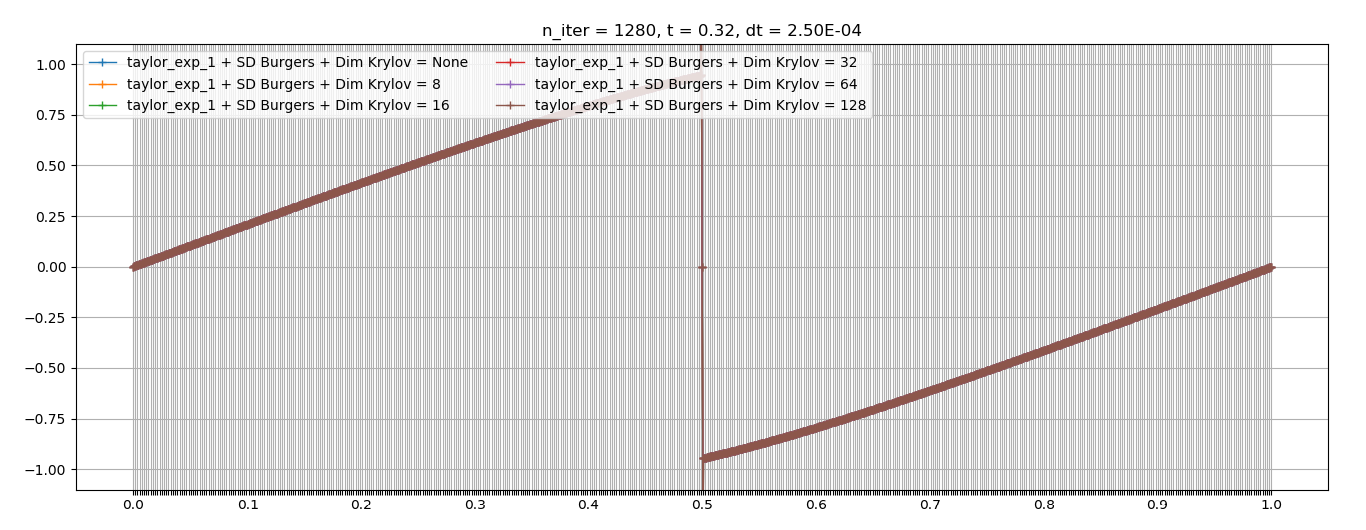
\includegraphics[width=\textwidth]{images/KrylovBurgers.png}
        \caption{Apparition d'une discontinuité dans la solution de l'équation de Burgers avec une condition initiale sinusoïdale, avec $\Delta t = 2.5e-4$, différences spectrales d'ordre 2 sur 511 cellules, exponentielle standard Taylor à l'ordre 1}
        \label{fig:BurgersKrylov}
\end{figure}

\begin{figure}[h!]
        \centering
        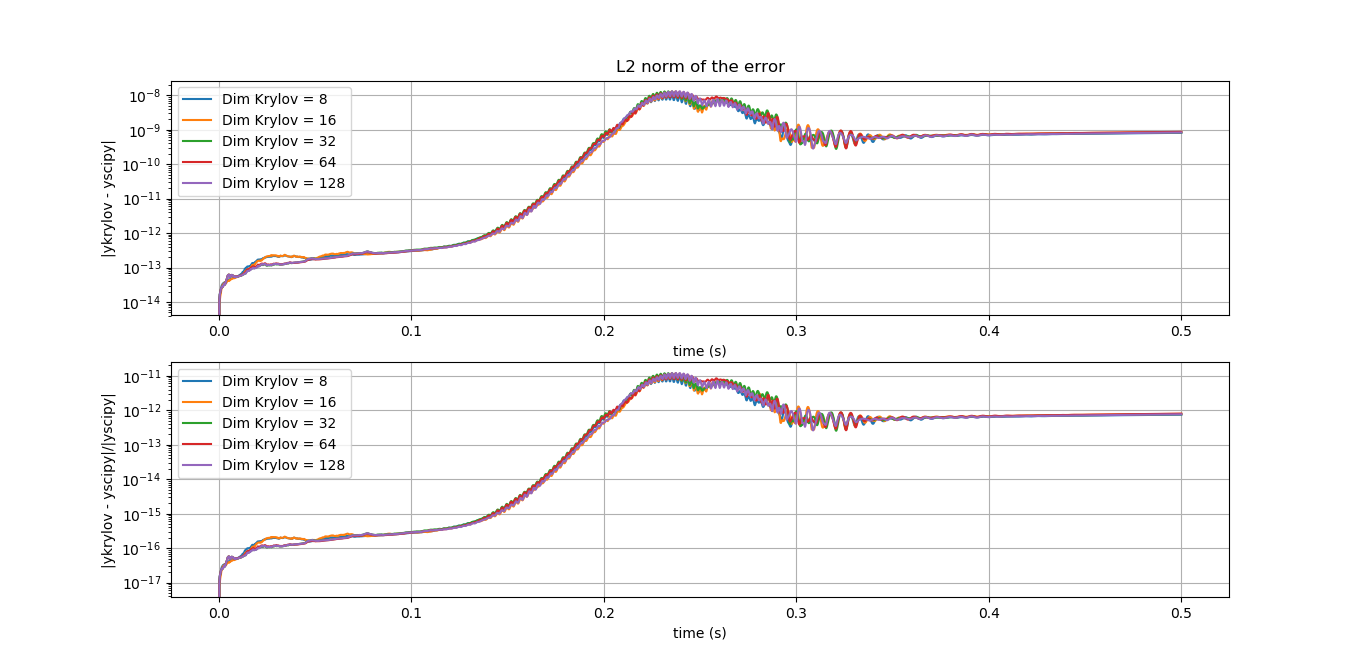
\includegraphics[width=\textwidth]{images/ErreurKrylov.png}
        \caption{Erreur absolue et relative associée à la méthode de Krylov sur l'exemple de la figure \ref{fig:BurgersKrylov}}
        \label{fig:Krylov}
\end{figure}

\begin{table}[h!]
\centering
\begin{tabular}{c|c|c|c|c|c|c|}
\cline{2-7}                            & \multicolumn{1}{c|}{\cellcolor[HTML]{C0C0C0}Scipy} & \multicolumn{1}{c|}{\cellcolor[HTML]{C0C0C0}m = 128} & \multicolumn{1}{c|}{\cellcolor[HTML]{C0C0C0}m = 64} & \multicolumn{1}{c|}{\cellcolor[HTML]{C0C0C0}m = 32} & \multicolumn{1}{c|}{\cellcolor[HTML]{C0C0C0}m = 16} & \multicolumn{1}{c|}{\cellcolor[HTML]{C0C0C0}m = 8} \\ \hline
\multicolumn{1}{|l|}{\cellcolor[HTML]{EFEFEF}temps (s)} & 2726.51 & 90.72 & 109.37 & 145.05 & 225.38 & 458.13 \\ \hline
\end{tabular}
\caption{Temps de calcul associés à l'exemple de la figure \ref{fig:BurgersKrylov}}
\label{tab:Krylov}
\end{table}

\paragraph{}
La première et, probablement, principale remarque est issue du tableau \ref{tab:Krylov} : l'applicabilité des méthodes exponentielles est indissociablement liée à l'utilisation des méthodes de Krylov. Même en 1D et avec une dimension assez réduite, si on cherche à résoudre le problème uniquement à l'aide de la méthode utilisée par Scipy, on obtient des temps de calcul trop élevés pour un code dont un des objectifs est l'application industrielle.

\paragraph{}
On se rend compte aussi que dans ce cas précis les erreurs obtenues, aussi bien celles absolues que celles relatives, restent très faibles au cours du temps. Plusieurs cas test exhibent des comportements très variés qui échappent encore à notre compréhension et pour lesquels nous n'avons pas encore pu trouver d'explication satisfaisante.

\paragraph{}
Il convient d'attirer l'attention sur le fait que, bien que cela ne soit pas clairement visible sur le graphe à cause de la superposition des courbes, l'algorithme utilisée par Scipy n'est pas exempt d'erreurs. Celles-ci semblent se concentrer sur la zone où se situe la discontinuité. Toutefois, on se focalise ici uniquement sur la mesure des écarts occasionnés par le calcul des exponentielles en fonction de la méthode utilisée. 

\paragraph{}
Il est aussi important de relever que dans l'exemple choisi, la condition CFL est inférieure à 1. Puisqu'un des avantages des méthodes exponentielles est leur stabilité accrue par rapport aux méthodes classiques, il peut être intéressant de savoir si  celle-ci peut être réduite à cause de l'utilisation de la méthode de Krylov. En augmentant le pas de temps progressivement, on voit que, sur l'exemple choisi, le domaine de stabilité, qui est en soi assez petit ($CFL \simeq 1.35$) à cause de la discontinuité, n'est pas affecté par l'utilisation de la méthode de Krylov.

\paragraph{}
On préconise la réalisation de tests supplémentaires pour confirmer les conclusions présentées ici et l'approfondissement sur l'analyse.

